\documentclass[11pt,a4paper]{article}

%--- Page + typography
\usepackage[margin=1.6cm]{geometry}
\usepackage{parskip}        % space between paragraphs
\usepackage{graphicx}       % for images (optional)
\usepackage{tabularx}       % flexible width tables
\usepackage{xcolor}
\usepackage{enumitem}       % compact lists
\usepackage{titlesec}       % tighter headings
\usepackage{tcolorbox}      % image placeholders
\usepackage{multicol}       % optional multi-column blocks
\usepackage{setspace}
\usepackage{wrapfig}

\setlist[itemize]{left=0pt, itemsep=2pt, topsep=2pt}

%--- A subtle header rule
\newcommand{\headerline}{\rule{\linewidth}{0.6pt}}

%--- A reusable placeholder for images (compiles without files)
% To use a real image instead, replace the entire tcolorbox with:
% \begin{center}\includegraphics[width=\linewidth]{your-image-file}\end{center}
\newtcolorbox{imgbox}[1][]{
  colback=black!3, colframe=black!35,
  boxrule=0.5pt, arc=2mm, left=3mm, right=3mm, top=2mm, bottom=2mm,
  fonttitle=\bfseries, title={#1}
}

%--- Compact Q/A item macro (keeps vertical footprint small)
\newcommand{\qa}[2]{\noindent\textbf{#1}\enspace #2\par}

\begin{document}
\pagestyle{empty}

\small % keeps everything neat on one A4 page

%================== HEADER ==================
Zhongyi Li \hfill \emph{To what extent is objectivity possible in the production or acquisition of knowledge?}\\

\vspace{4pt}

%================== OBJECT 1 ==================
\section{Lecture ``On Mathematical Maturity'' (Thomas Garrity)}
\ 
\begin{wrapfigure}{r}{0.38\textwidth}
  \begin{center}
    \includegraphics[width=0.35\textwidth]{functions.jpg}
  \end{center}
\end{wrapfigure}

\qa{What is the object?}{A recorded lecture by mathematician Thomas Garrity on ``mathematical maturity.''}
\qa{Real-world context / history:}{Delivered in 2017 to undergraduates and K–12 educators, the talk frames mathematical maturity as the intuition and creativity needed to tackle unfamiliar problems.}
\qa{Relation to the prompt:}{While published proofs in mathematics are objective, the \emph{production} of such knowledge relies on subjective elements (intuition, pattern-spotting, abstraction). Hence, mathematics blends an objective end state with subjective means, limiting complete objectivity in its creation.}

\vspace{6pt}
\headerline
\vspace{4pt}

%================== OBJECT 2 ==================
\section{Gua Sha Tool (Traditional Chinese Medicine)}
\ 
\begin{wrapfigure}{l}{0.38\textwidth}
  \begin{center}
    \includegraphics[width=0.35\textwidth]{guasha.jpg}
  \end{center}
\end{wrapfigure}

\qa{What is the object?}{A scraping tool used in Traditional Chinese Medicine (TCM), believed to “release toxins.”}
\qa{Real-world context / history:}{Practiced for centuries and transmitted culturally (e.g., gifted within families), Gua Sha persists despite a lack of support from evidence-based biomedicine and known risks like skin damage.}
\qa{Relation to the prompt:}{Scientific medicine aims at objectivity through falsifiability, controls, and statistics; TCM often appeals to tradition and anecdote. Divergent standards of justification reveal how cultural commitments constrain the attainment and spread of objective medical knowledge.}

\vspace{6pt}
\headerline
\vspace{4pt}

%================== OBJECT 3 ==================
\section{Ravel — \emph{Piano Concerto for the Left Hand in D major}}
\ 
\begin{wrapfigure}{r}{0.38\textwidth}
  \begin{center}
    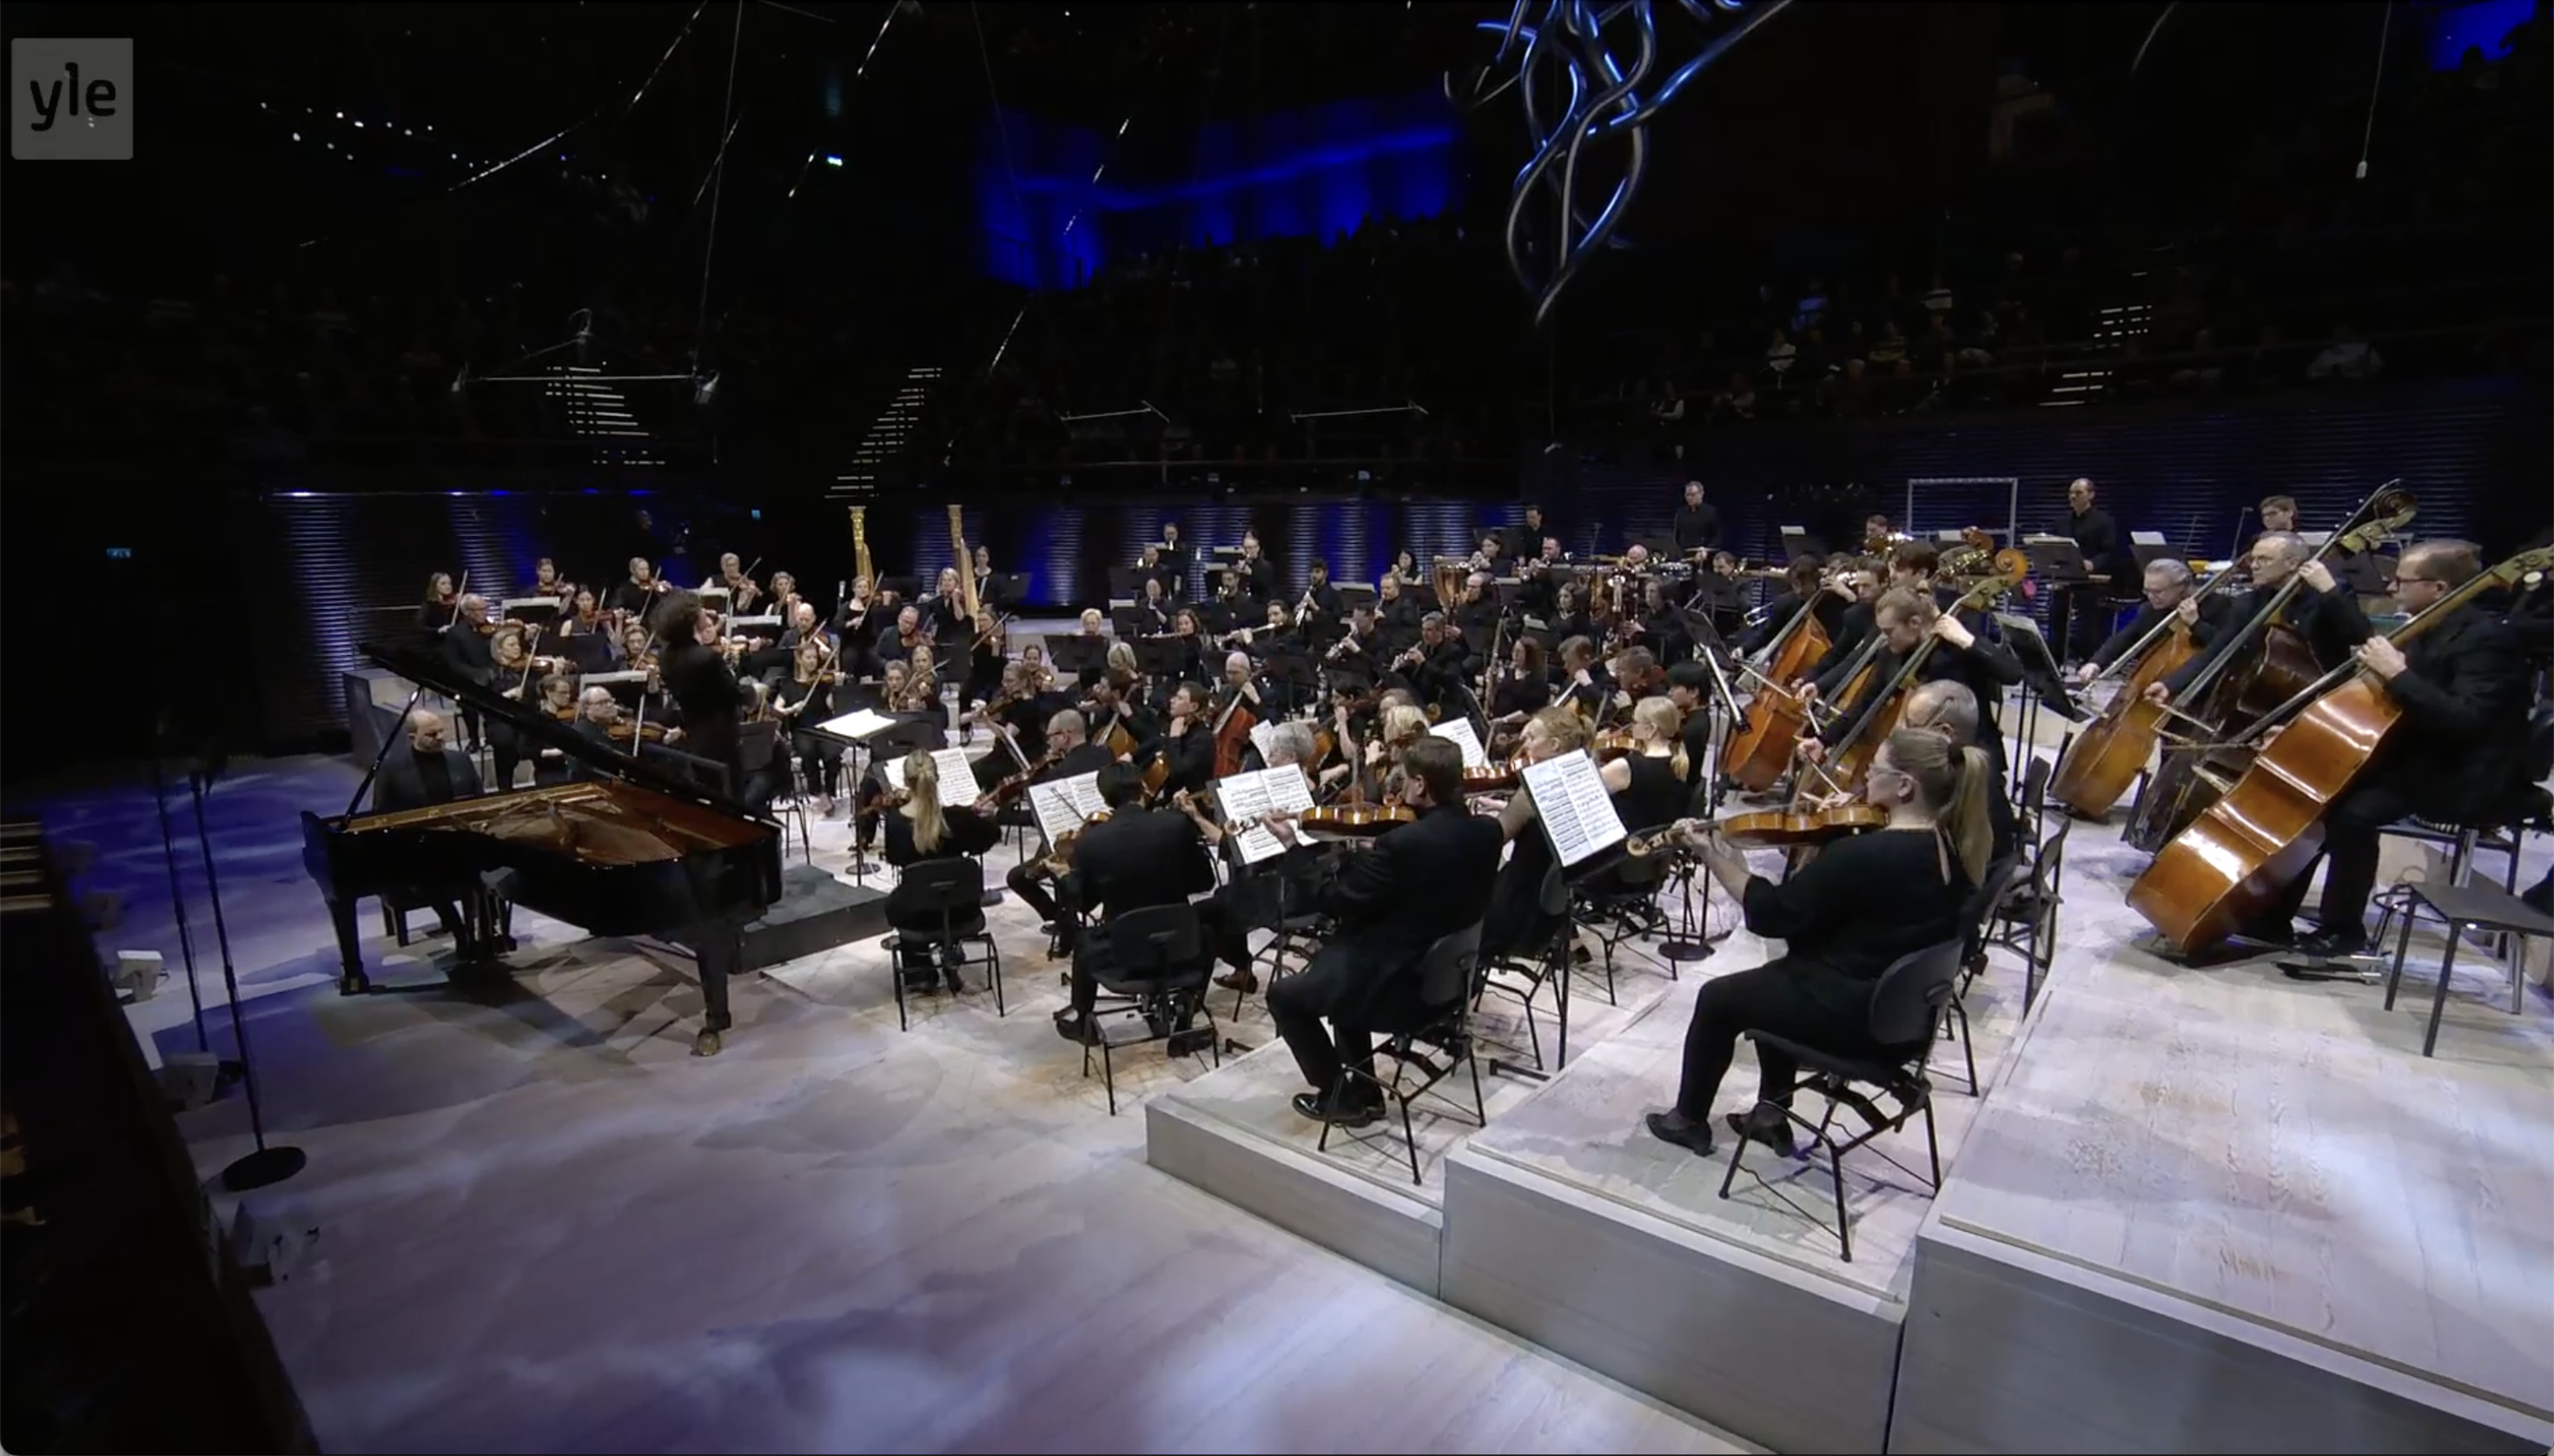
\includegraphics[width=0.35\textwidth]{music}
  \end{center}
\end{wrapfigure}

\qa{What is the object?}{A concerto composed by Maurice Ravel for pianist Paul Wittgenstein, who lost his right hand in World War~I.}
\qa{Real-world context / history:}{Popular summaries cast it as an inspiring gesture of compassion; in fact, it was a paid commission, and later disputes arose over Wittgenstein's departures from Ravel's score.}
\qa{Relation to the prompt:}{Short-form, emotionally charged retellings simplify and omit complexities, shaping what audiences “know.” Historical knowledge is filtered through selection and perspective, so complete objectivity in history is elusive.}
\vfill
\tiny{\color{gray!20}The source code for this PDF is almost completely generated by GPT5 based on my TOK exhibition final draft. I am very impressed and satisfied with its capability.}
\end{document}